\chapter{Planificación de caja}\label{chp-04}

Para que todos los dispositivos que componen el sistema estén bien aislados del exterior
y no haya problemas con las conexiones se planifica una caja estanca. Ésta deberá ser 
accesible para el reemplazo de dispositivos defectuosos y ser replicable. 

\section{Diseño de caja}

Como referencia se toma de una caja de dimensiones 220 x 145 x 80 mm. Para reducir los 
costes, se decide imprimirla en 3D, ya que permite mayor adaptabilidad para colocar 
los lugares donde fijar los diferentes dispositivos. La caja estará dividida en una base y una 
tapa que se unen mediante tornillos y permiten una unión estable.

\subsection{Base}



\begin{figure}[htpb]% 
    \centering 
    \subfloat[][]{% 
        \label{fig:cajabasevista}% 
        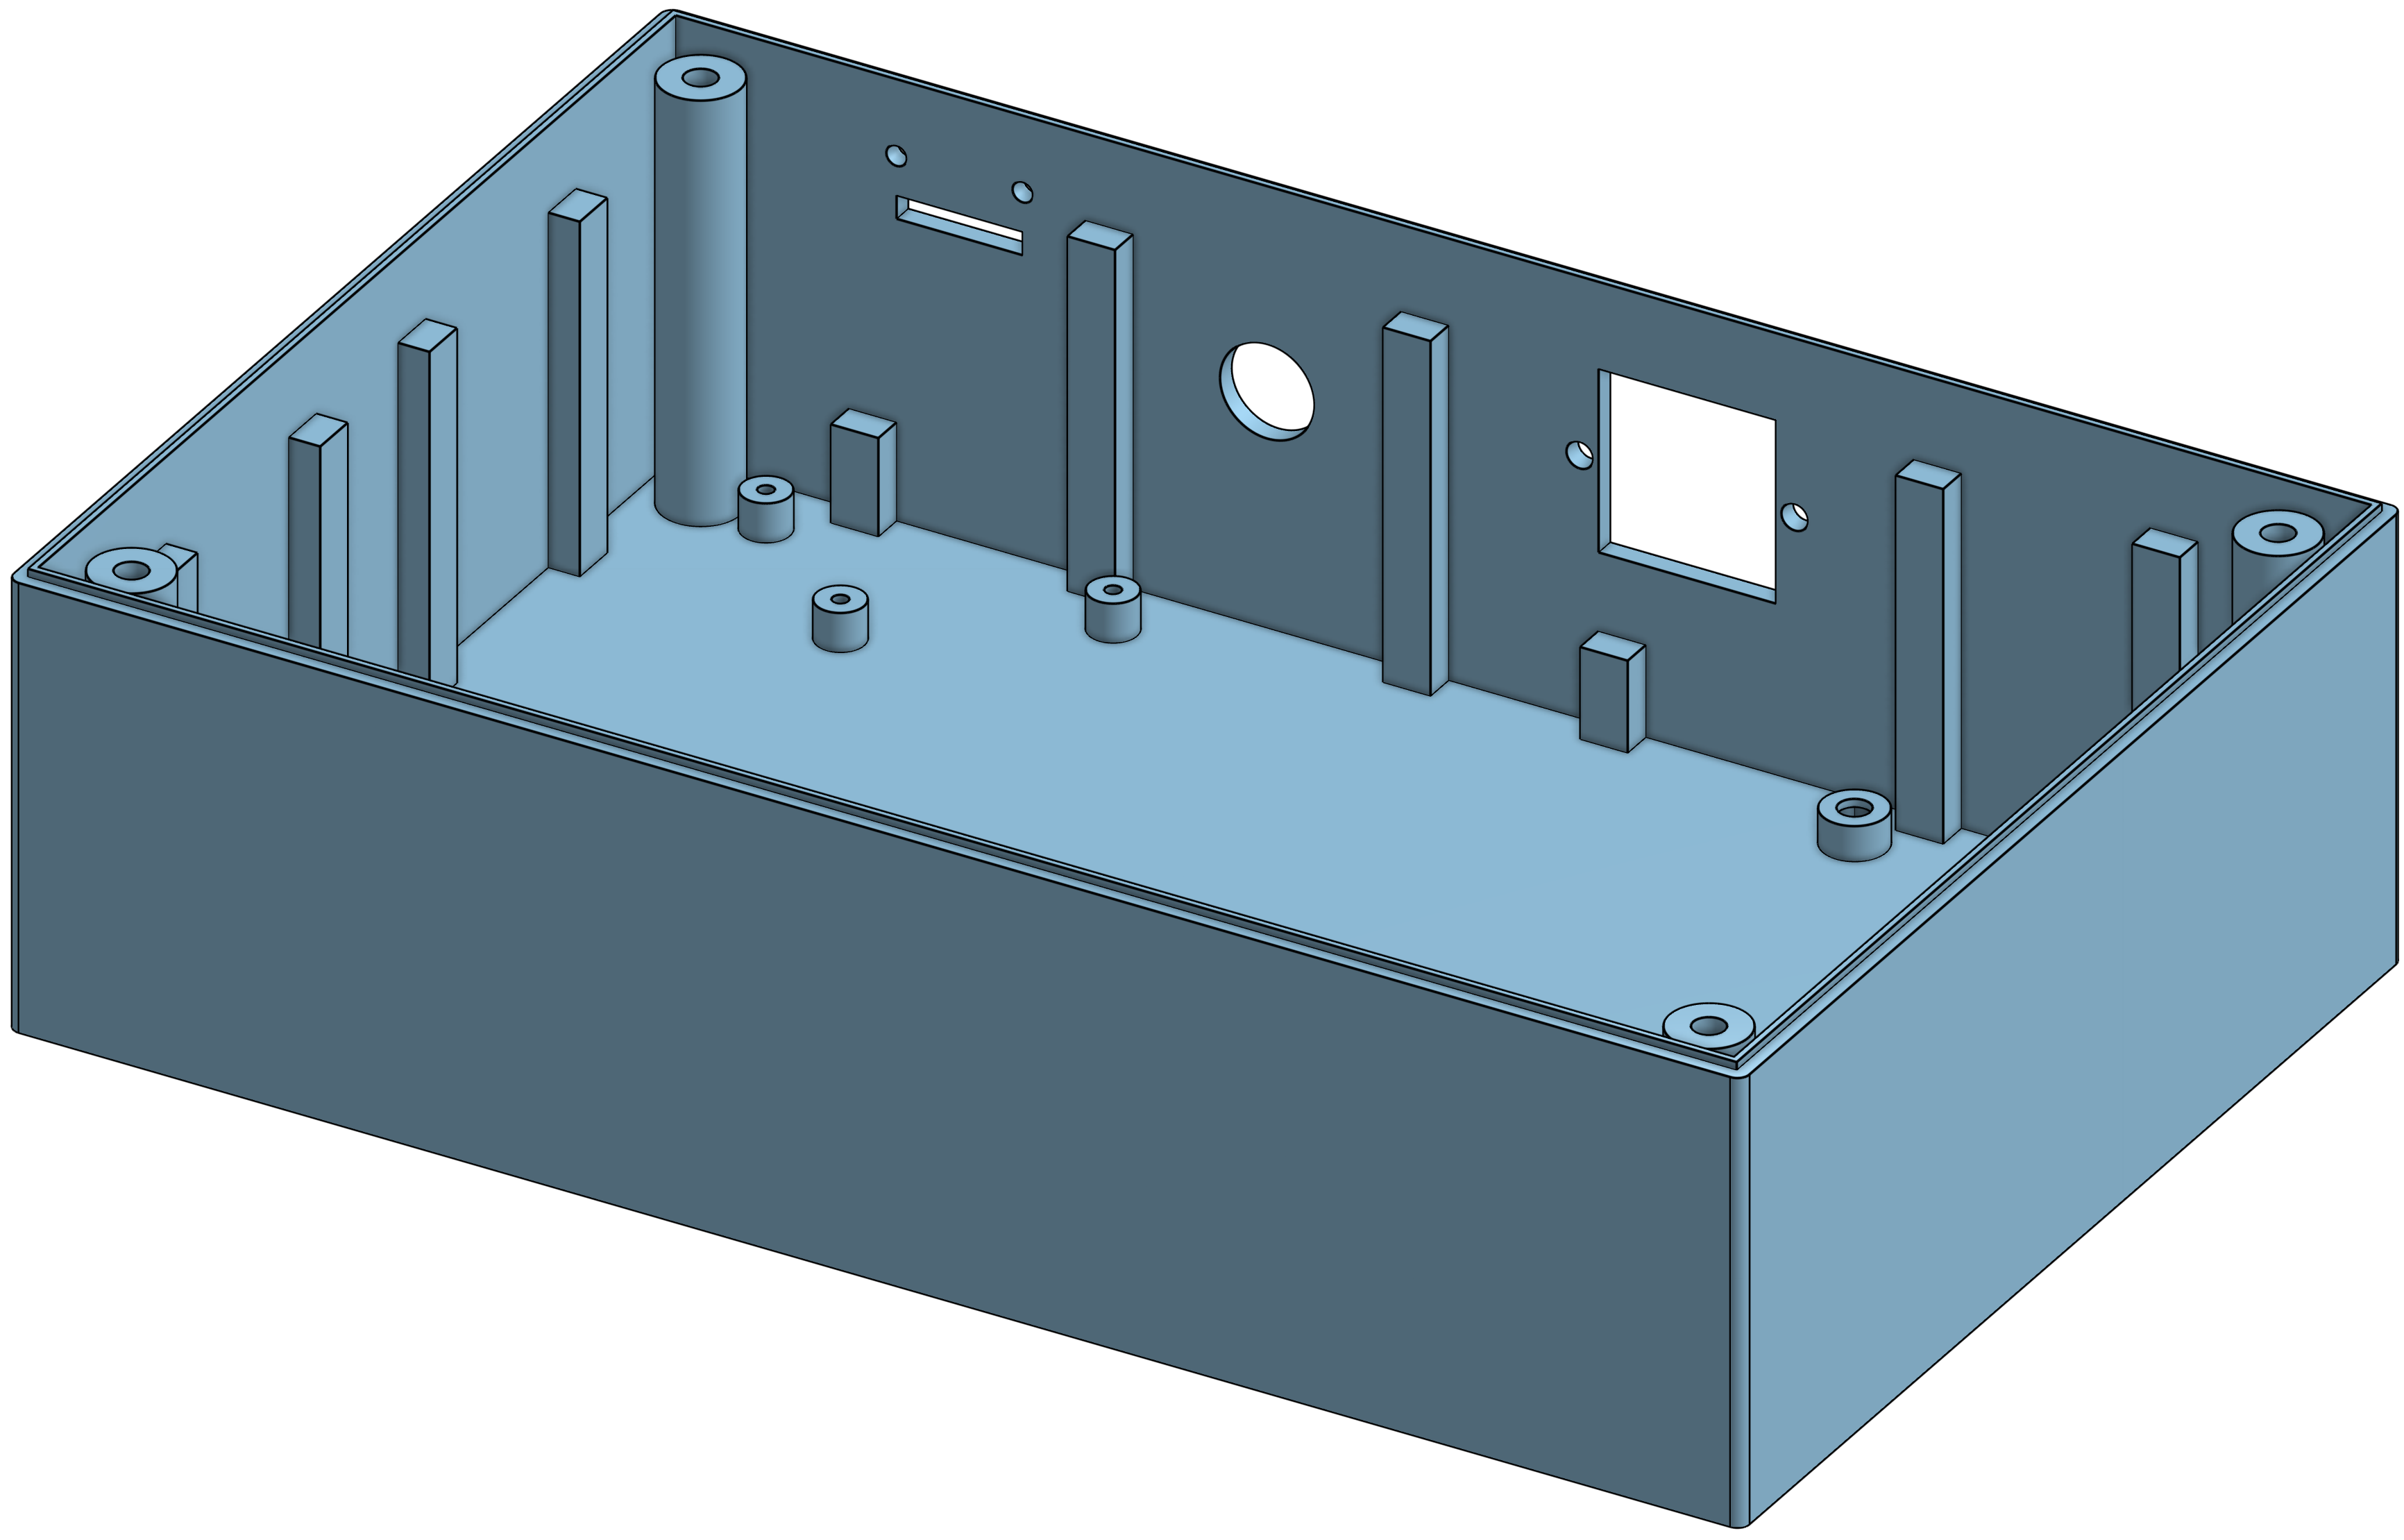
\includegraphics[width=0.75\textwidth]{04-caja/cajabase.png}
    }% 
    \hspace{10pt}% 
    \subfloat[][]{% 
        \label{fig:cajabaseplanta}% 
        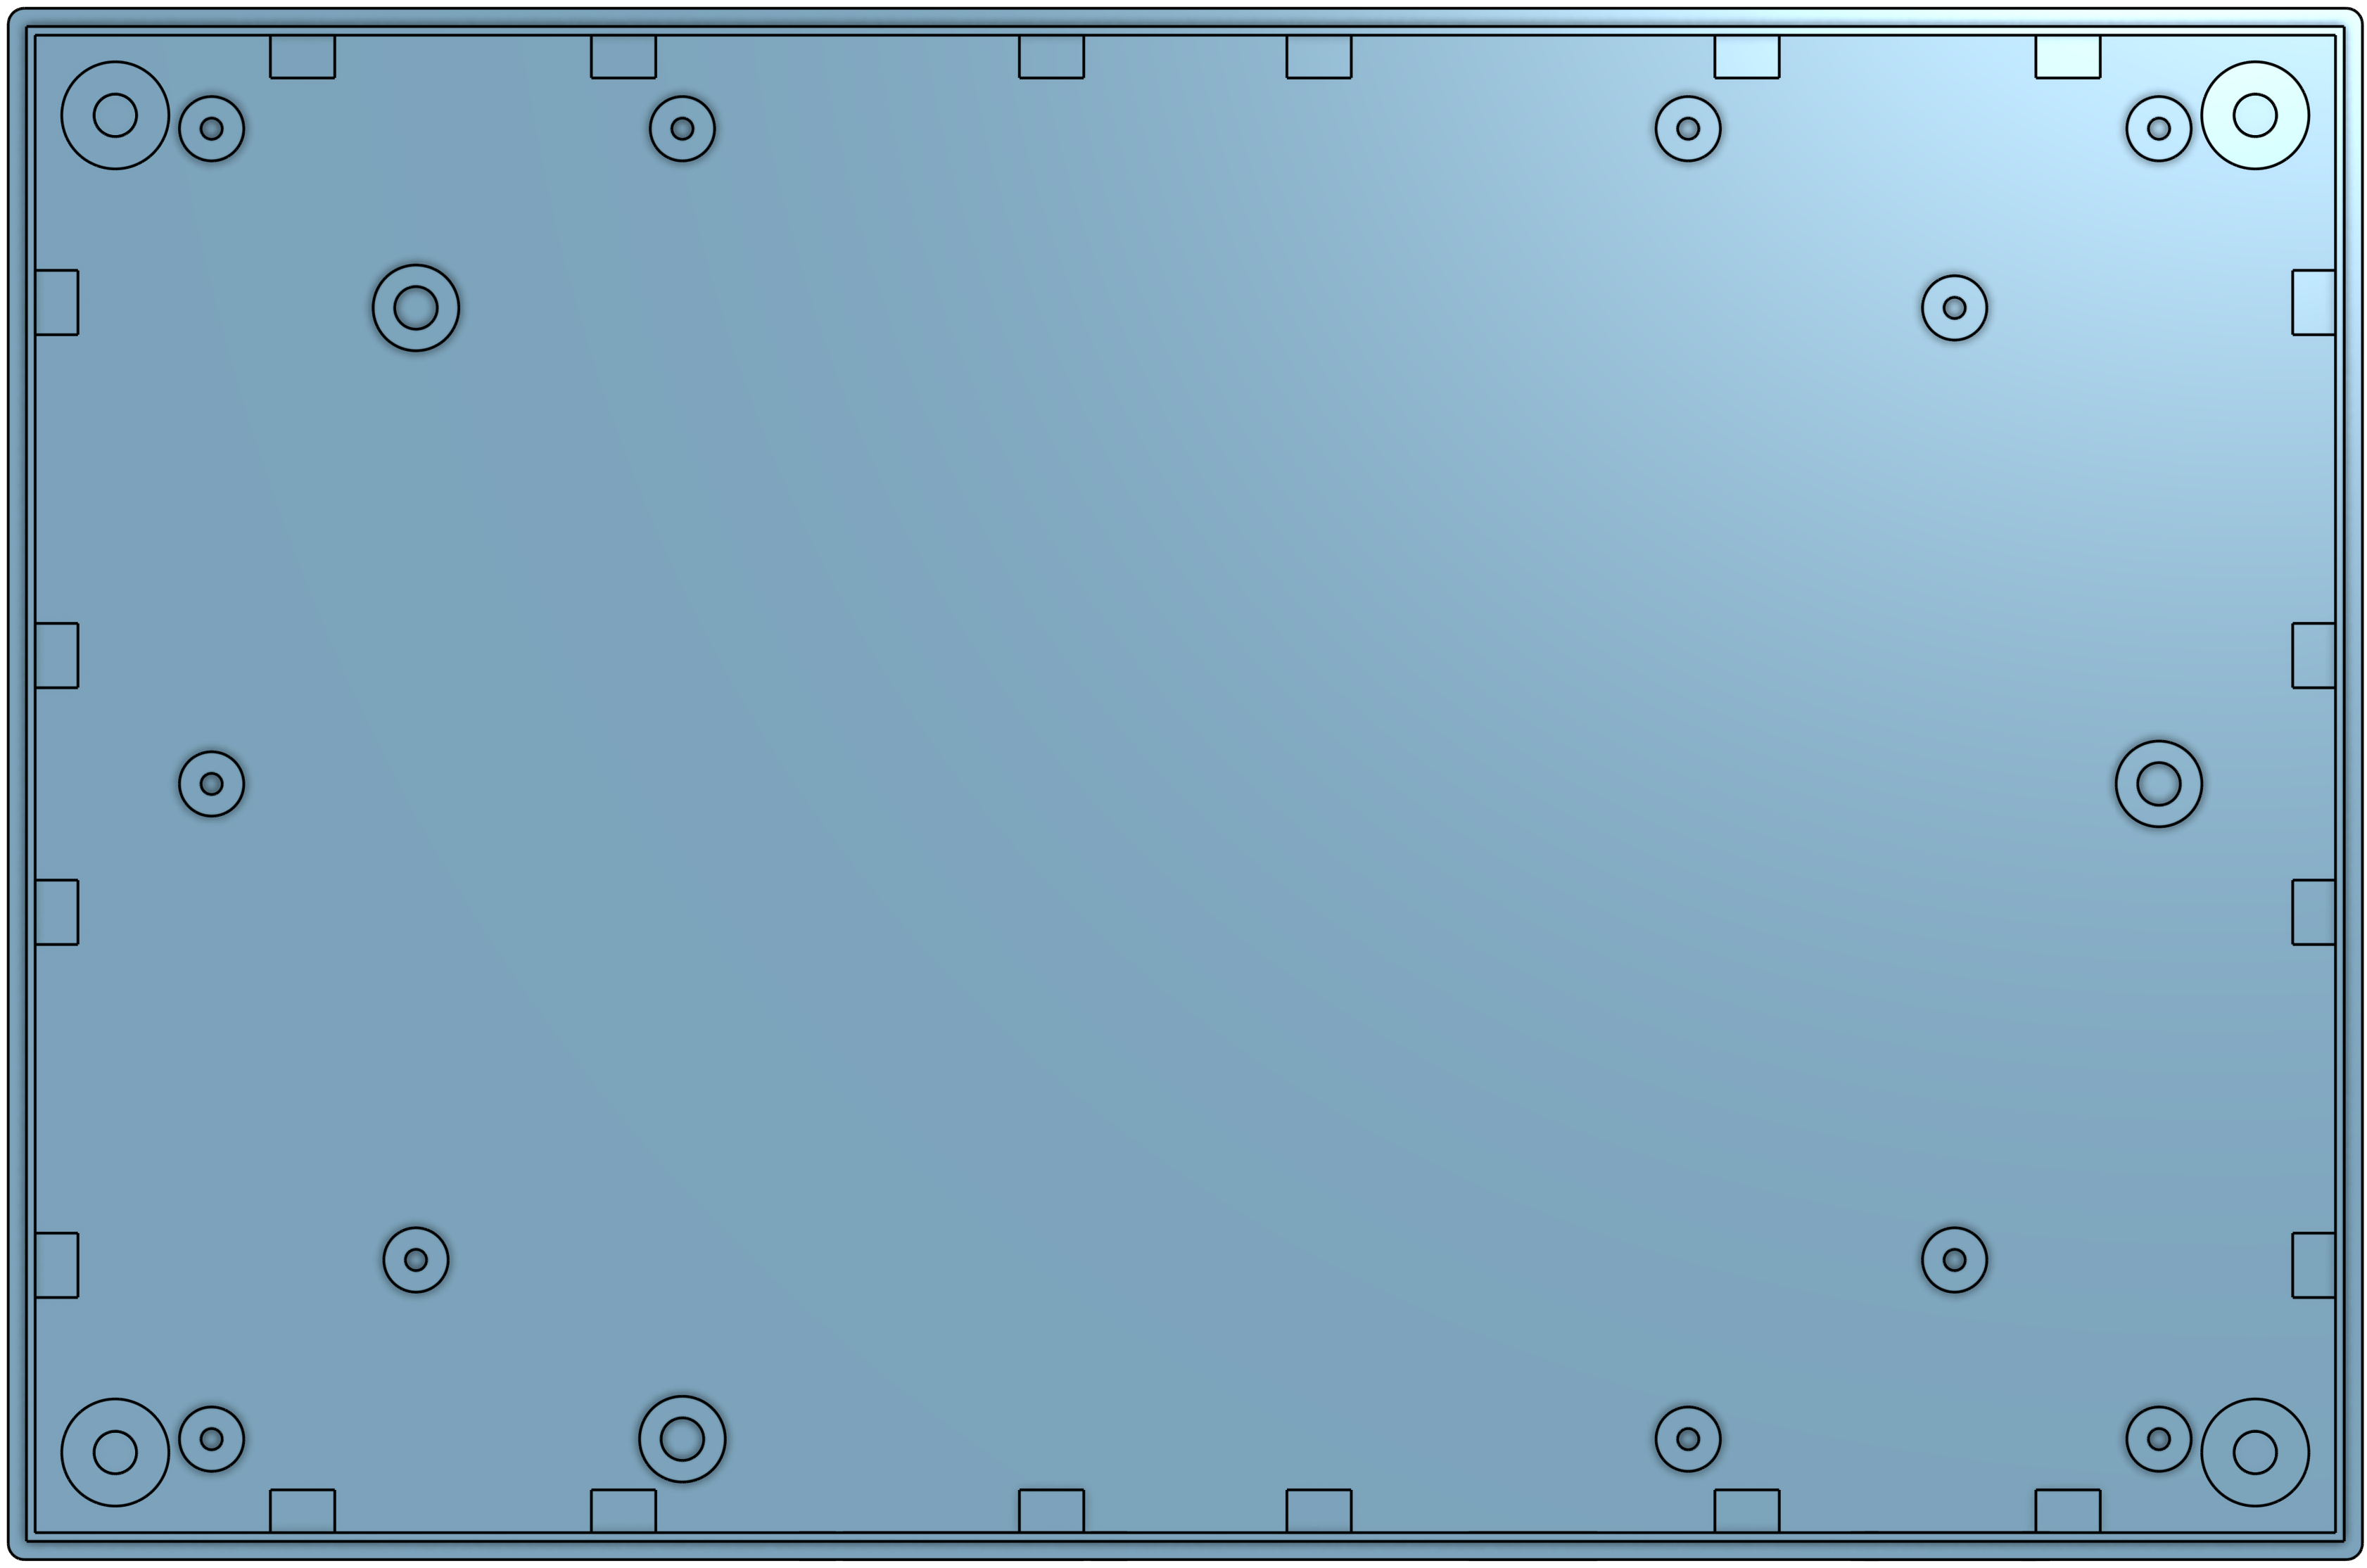
\includegraphics[width=0.75\textwidth]{04-caja/cajabaseplanta.png}
    }
    \caption{a) Vista general de la base de la caja. b) Vista de planta de la base de la caja}
    \label{fig:cajabase} 
\end{figure} 

\subsection{Tapa}

\begin{figure}[htpb]% 
    \centering 
    \subfloat[][]{% 
        \label{fig:cajatapavista}% 
        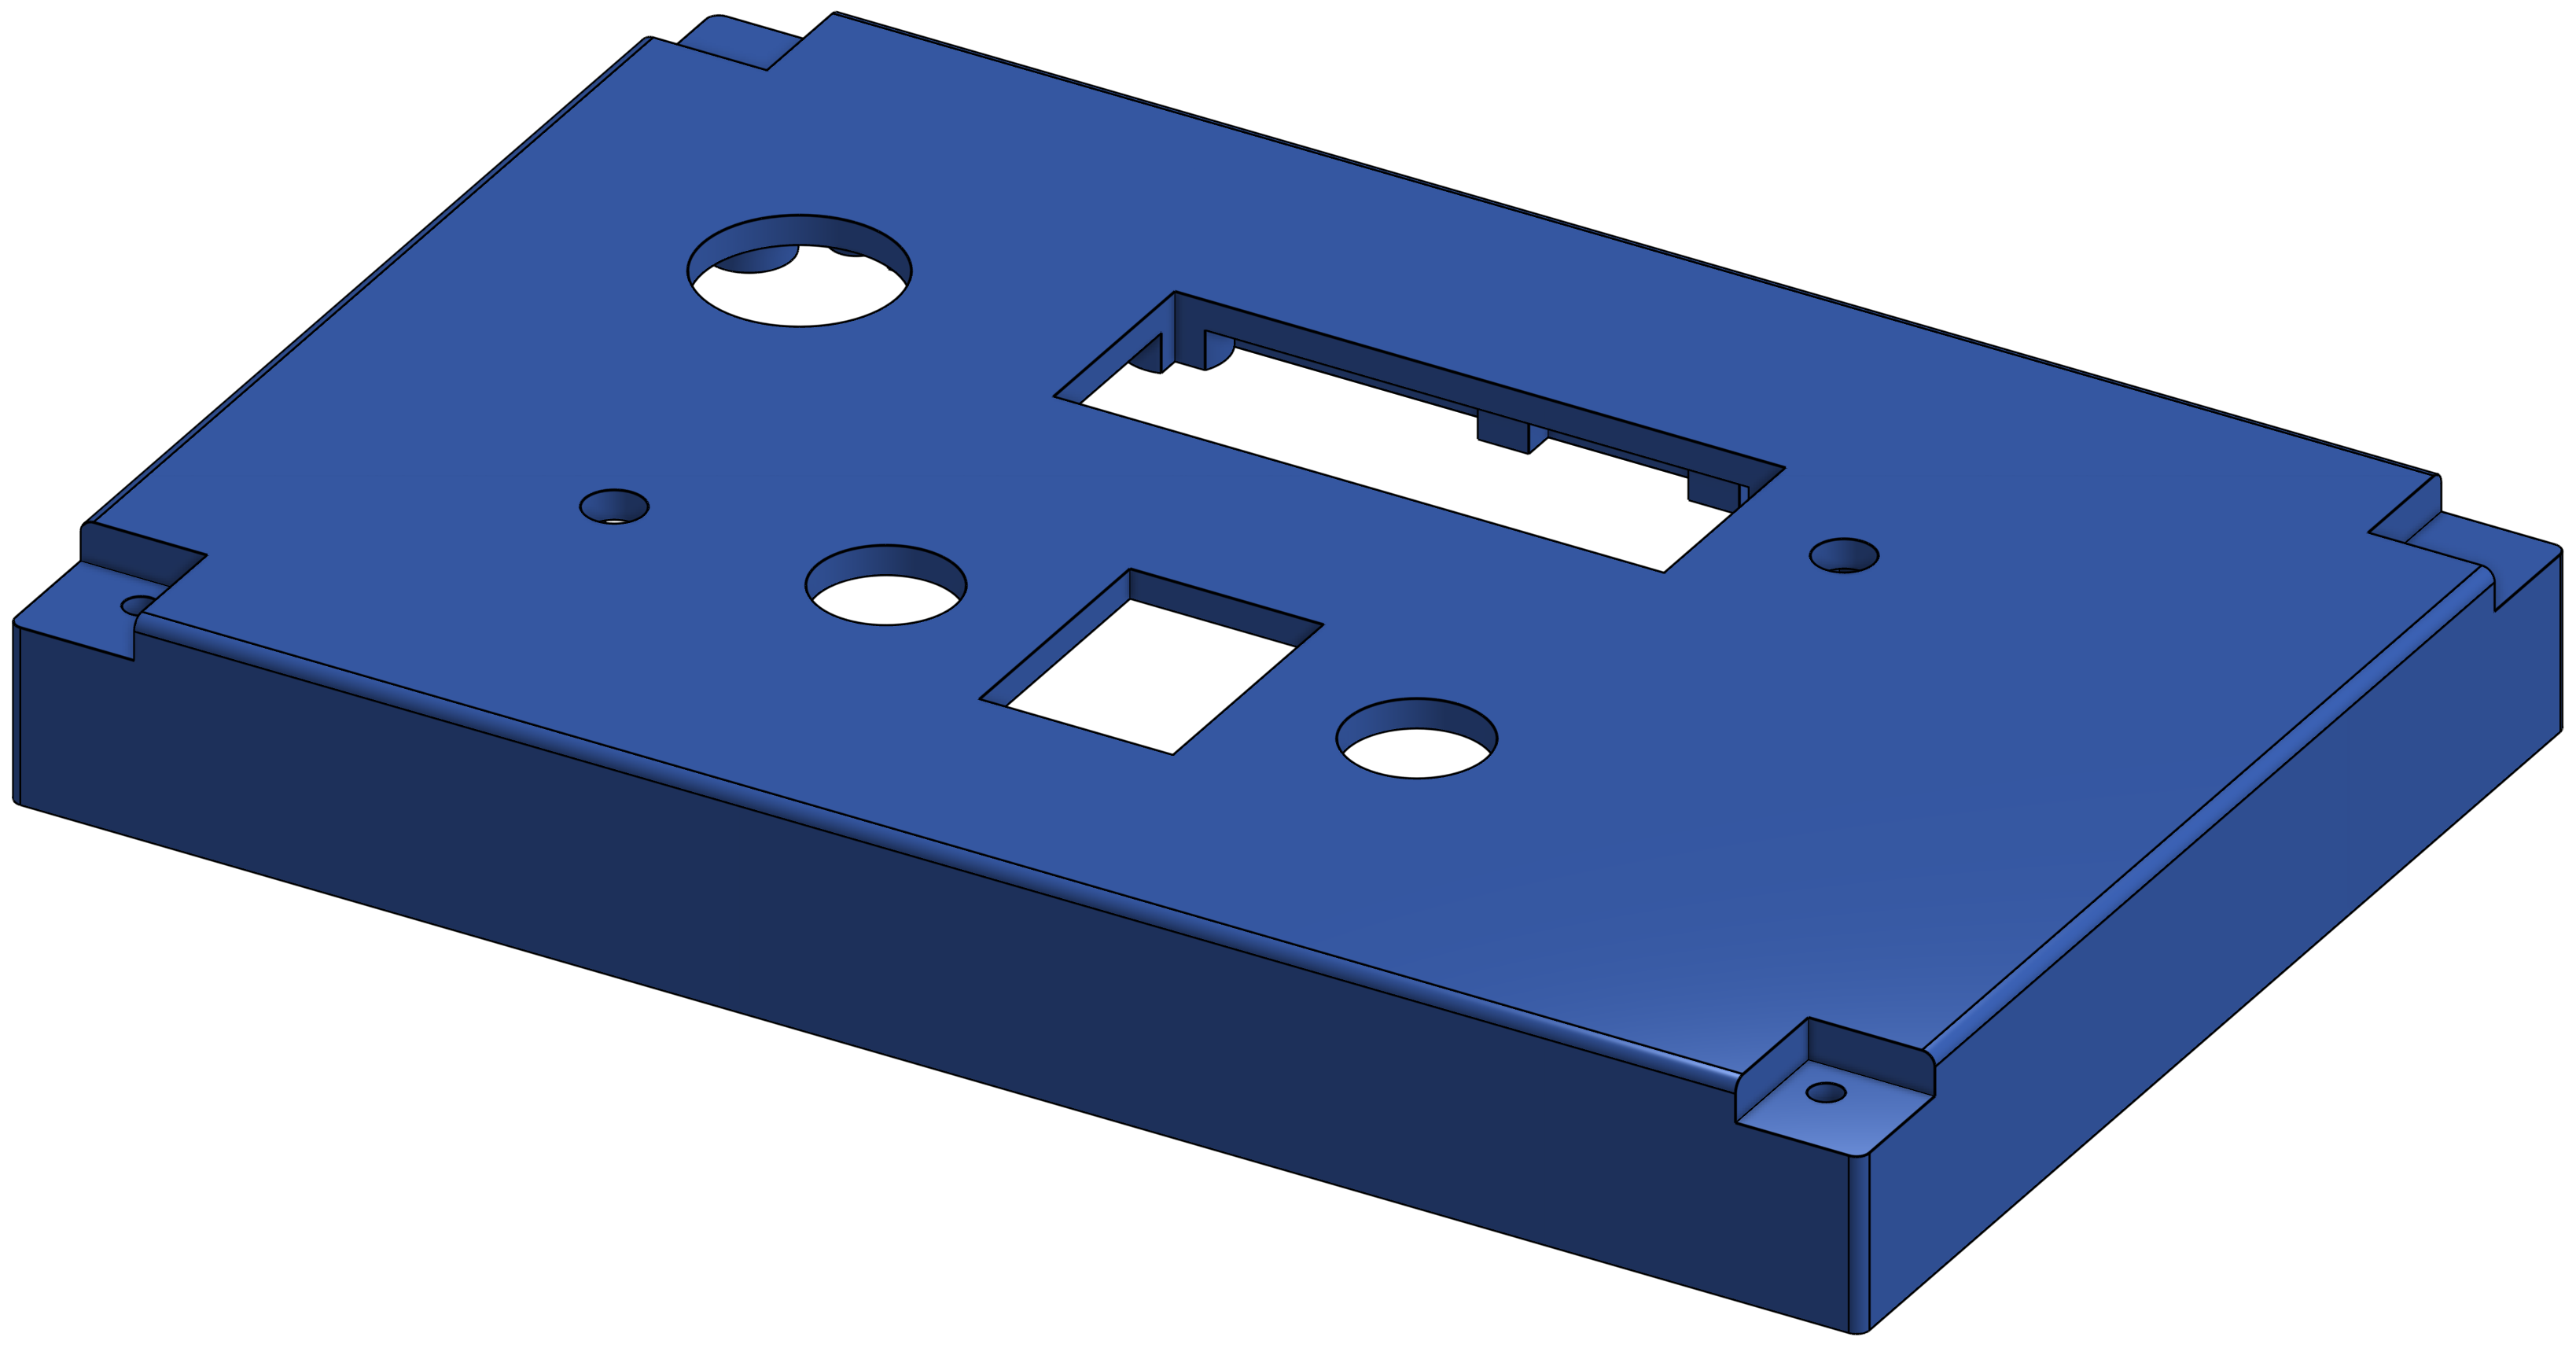
\includegraphics[width=0.75\textwidth]{04-caja/cajatapa.png}
    }% 
    \hspace{10pt}% 
    \subfloat[][]{% 
        \label{fig:cajatapaplanta}% 
        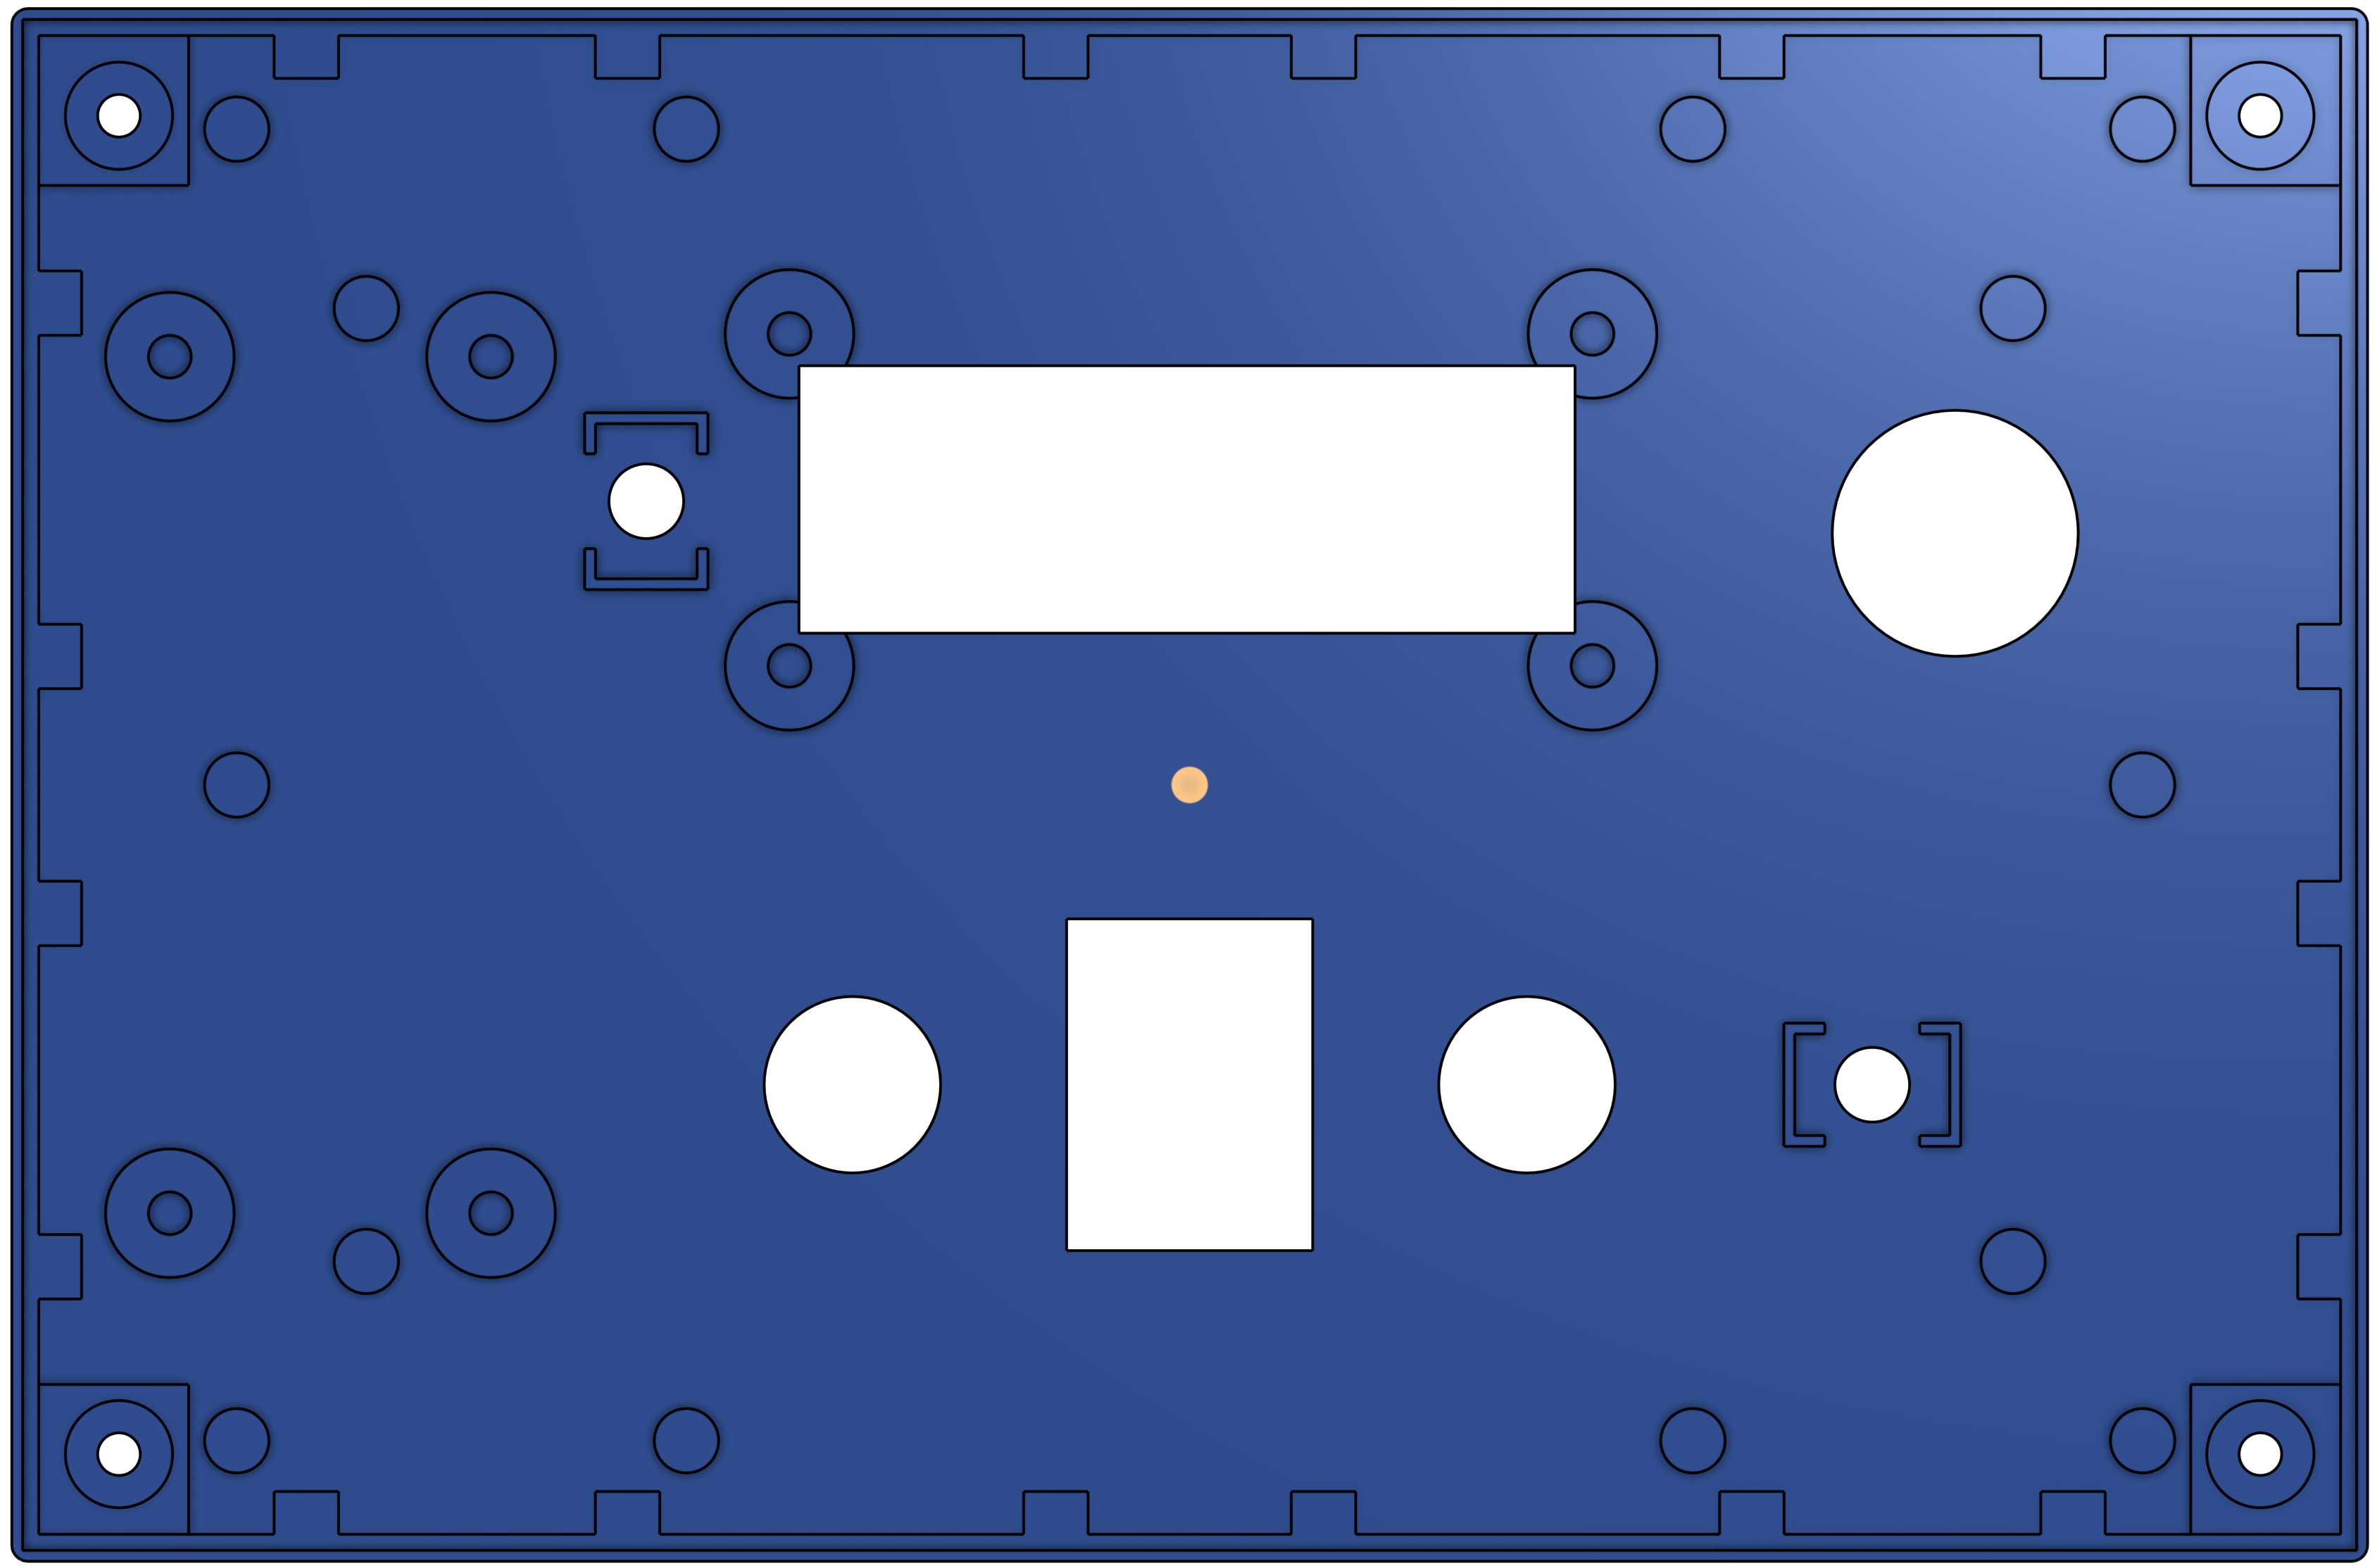
\includegraphics[width=0.75\textwidth]{04-caja/cajatapafondo.png}
    }
    \caption{a) Vista general de la tapa de la caja. b) Vista inferior de la tapa de la caja}
    \label{fig:cajatapa} 
\end{figure} 
